\documentclass[11pt,reqno,final,pdftex]{amsart}\usepackage[]{graphicx}\usepackage[]{color}
%% maxwidth is the original width if it is less than linewidth
%% otherwise use linewidth (to make sure the graphics do not exceed the margin)
\makeatletter
\def\maxwidth{ %
  \ifdim\Gin@nat@width>\linewidth
    \linewidth
  \else
    \Gin@nat@width
  \fi
}
\makeatother

\definecolor{fgcolor}{rgb}{0.345, 0.345, 0.345}
\newcommand{\hlnum}[1]{\textcolor[rgb]{0.686,0.059,0.569}{#1}}%
\newcommand{\hlstr}[1]{\textcolor[rgb]{0.192,0.494,0.8}{#1}}%
\newcommand{\hlcom}[1]{\textcolor[rgb]{0.678,0.584,0.686}{\textit{#1}}}%
\newcommand{\hlopt}[1]{\textcolor[rgb]{0,0,0}{#1}}%
\newcommand{\hlstd}[1]{\textcolor[rgb]{0.345,0.345,0.345}{#1}}%
\newcommand{\hlkwa}[1]{\textcolor[rgb]{0.161,0.373,0.58}{\textbf{#1}}}%
\newcommand{\hlkwb}[1]{\textcolor[rgb]{0.69,0.353,0.396}{#1}}%
\newcommand{\hlkwc}[1]{\textcolor[rgb]{0.333,0.667,0.333}{#1}}%
\newcommand{\hlkwd}[1]{\textcolor[rgb]{0.737,0.353,0.396}{\textbf{#1}}}%

\usepackage{framed}
\makeatletter
\newenvironment{kframe}{%
 \def\at@end@of@kframe{}%
 \ifinner\ifhmode%
  \def\at@end@of@kframe{\end{minipage}}%
  \begin{minipage}{\columnwidth}%
 \fi\fi%
 \def\FrameCommand##1{\hskip\@totalleftmargin \hskip-\fboxsep
 \colorbox{shadecolor}{##1}\hskip-\fboxsep
     % There is no \\@totalrightmargin, so:
     \hskip-\linewidth \hskip-\@totalleftmargin \hskip\columnwidth}%
 \MakeFramed {\advance\hsize-\width
   \@totalleftmargin\z@ \linewidth\hsize
   \@setminipage}}%
 {\par\unskip\endMakeFramed%
 \at@end@of@kframe}
\makeatother

\definecolor{shadecolor}{rgb}{.97, .97, .97}
\definecolor{messagecolor}{rgb}{0, 0, 0}
\definecolor{warningcolor}{rgb}{1, 0, 1}
\definecolor{errorcolor}{rgb}{1, 0, 0}
\newenvironment{knitrout}{}{} % an empty environment to be redefined in TeX

\usepackage{alltt}
%% DO NOT DELETE OR CHANGE THE FOLLOWING TWO LINES!
%% $Revision$
%% $Date$
\usepackage[round,sort,elide]{natbib}
\usepackage{graphicx}
\usepackage{times}
\usepackage{rotating}
\usepackage{subfig}
\usepackage{color}
\newcommand{\aak}[1]{\textcolor{cyan}{#1}}
\newcommand{\mab}[1]{\textcolor{red}{#1}}
\newcommand{\cec}[1]{\textcolor{blue}{#1}}

\setlength{\textwidth}{6.25in}
\setlength{\textheight}{8.75in}
\setlength{\evensidemargin}{0in}
\setlength{\oddsidemargin}{0in}
\setlength{\topmargin}{-.35in}
\setlength{\parskip}{.1in}
\setlength{\parindent}{0.3in}

%% cleveref must be last loaded package
\usepackage[sort&compress]{cleveref}
\crefname{figure}{Fig.}{Figs.}
\Crefname{figure}{Fig.}{Figs.}
\crefname{table}{Table}{Tables}
\Crefname{table}{Tab.}{Tables}
\crefname{equation}{Eq.}{Eqs.}
\Crefname{equation}{Eq.}{Eqs.}
\crefname{appendix}{Appendix}{Appendices}
\Crefname{appendix}{Appendix}{Appendices}
\creflabelformat{equation}{#2#1#3}
\newcommand{\crefrangeconjunction}{--}
\newcommand{\creflastconjunction}{, and~}

\theoremstyle{plain}
\newtheorem{thm}{Theorem}
\newtheorem{corol}[thm]{Corollary}
\newtheorem{prop}[thm]{Proposition}
\newtheorem{lemma}[thm]{Lemma}
\newtheorem{defn}[thm]{Definition}
\newtheorem{hyp}[thm]{Hypothesis}
\newtheorem{example}[thm]{Example}
\newtheorem{conj}[thm]{Conjecture}
\newtheorem{algorithm}[thm]{Algorithm}
\newtheorem{remark}{Remark}
\renewcommand\thethm{\arabic{thm}}
\renewcommand{\theremark}{}

\numberwithin{equation}{part}
\renewcommand\theequation{\arabic{equation}}
\renewcommand\thesection{\arabic{section}}
\renewcommand\thesubsection{\thesection.\arabic{subsection}}
\renewcommand\thefigure{\arabic{figure}}
\renewcommand\thetable{\arabic{table}}
\renewcommand\thefootnote{\arabic{footnote}}

\newcommand\scinot[2]{$#1 \times 10^{#2}$}
\newcommand{\code}[1]{\texttt{#1}}
\newcommand{\pkg}[1]{\textsf{#1}}
\newcommand{\dlta}[1]{{\Delta}{#1}}
\newcommand{\Prob}[1]{\mathbb{P}\left[#1\right]}
\newcommand{\Expect}[1]{\mathbb{E}\left[#1\right]}
\newcommand{\Var}[1]{\mathrm{Var}\left[#1\right]}
\newcommand{\dd}[1]{\mathrm{d}{#1}}
\newcommand{\citetpos}[1]{\citeauthor{#1}'s \citeyearpar{#1}}
\IfFileExists{upquote.sty}{\usepackage{upquote}}{}
\begin{document}



Okay, beginning to work on a macroparasite version of the energy budget model I proposed in the Ecol. Lett. paper.
The goal is to develop a general model for macroparasitic infection (with an eye towards helminthic parasites).
The hope would be to develop a model that could be extended to consider whipworm infections, so I will take up that problem at the end, by interpreting some early experimental returns in light of the general model.

The basic model structure is shown in Fig. \ref{fig:DEB_diagram}.
\begin{figure}
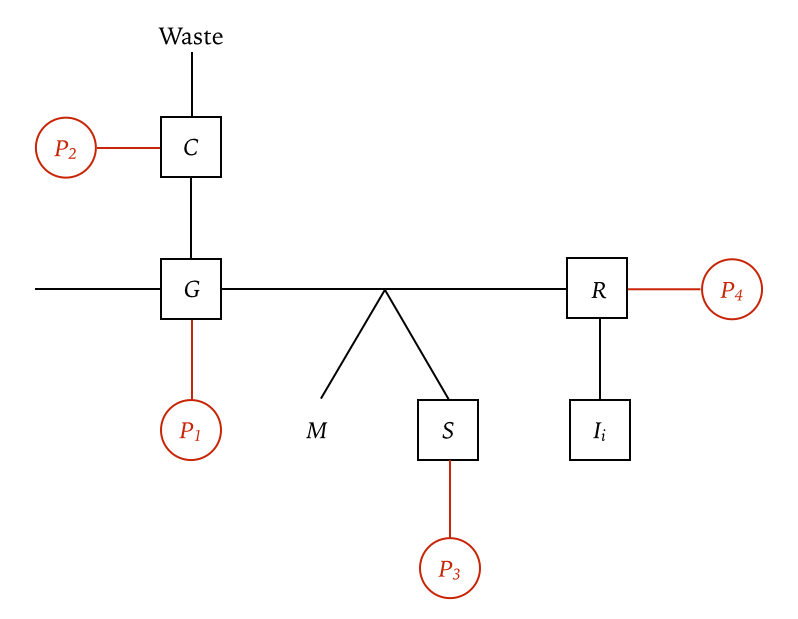
\includegraphics[width=\textwidth]{Macroparasite_DEB.png}
\caption{``Bins and flows'' model of host and parasite energetics. ``Bins'' are represented by the boxes in the diagram: biologically, these are places where energy is stored; mathematically, they are state variables of the model. Text without boxes represent ``flows'' of energy through (and out of) the host. See the text for a fuller description of the model.}
\label{fig:DEB_diagram}
\end{figure}

The host is assumed to ingest resources/energy at a rate $E_{ingest}$.
 fraction of this resource is assimilated $E_{assim}$ and is utilized by the host to fuel all metabolic processes; the remainder is lost as waste.
Out of the assimilated energy, maintenance (including the cost of constitutive immune defense) is paid first (making this a net production model of host energetics).
The remainder is allocated towards structure or fat reserves (which may be considered the reproduction buffer).
By structure, we mean investment in things like the skeleton that cannot be ``reclaimed'' during periods of starvation.
This is why fat reserves do not make up part of structure.
Reproduction is paid using the energy in the fat reserves, but so is the induced immune response.
The fact that the induced immune response depends on fat reserves has been shown empirically, as fat stores are known to provide places for lymphocytes to get organized, and leptin (a hormone produced in adipose tissue) helps regulate the induced immune response.
Parasites (represented by $P_i$ in the diagram) may tap into this energy budget in different places depending on the parasite.
Some ($P_1$) may steal energy before it has been assimilated into metabolizable energy by the host; tapeworms may be a good example of this kind of parasite.
Others ($P_2$) may use energy that is going to be excreted as waste; whipworms might be a good example here.
Interestingly, this would suggest that a good strategy for such a parasite is to reduce assimilation efficiency, which whipworms actually do.
A third category of parasites ($P_3$) take energy after maintenance has been paid, but before the energy has been allocated to growth and reproduction: this strategy has a benefit for the parasite of being less likely to induce starvation in the host (where starvation is defined as a situation where energy input is insufficient to meet maintenance demands).
I am not aware of any parasites that could be considered to be part of this class, but no doubt they exist.
Still other parasites ($P_4$) may use components of structure themselves as a resource.
For example, parasites that feed on tissue or blood could be considered parasites of structure.
Finally, some parasites ($P_5$) may use fat reserves as a resource.
Of course, some parasites might be considered to fall into more than one class.
Perhaps an example of this would be the trematode parasites of some snails that actually physically destroy the gonads.
Although those might more profitably be considered parasites of structure in this framework - they consume the gonads (a component of structure, in my opinion) which causes reproduction itself to stop.
Thus more energy is allocated to structure and/or fat reserves, which the parasites then utilize as a resource.

This basic stucture can be tweaked as necessary, for example, to consider multiple arms of the immune response (e.g., Th1/Th2) or to consider both growth and reproduction of parasites (which might require a more complicated model to track both parasite density and parasite size-structure within the host).

I also point out that the cells of the constitutive and induced immune response need not correspond exactly with how those cells are defined biologically.
For example, during an immune response to infection, lymphocytes (cells of the induced or adaptive immune system) can cause the production of more eosinophils (cells of the constitutive immune system).
In the model, however, we can consider these new eosinophils to be cells of the induced response.
Similarly, there are always lymphocytes around, and these cells should be considered in the model as cells of the constitutive immune system.

\subsection*{Other possible energy budget structures}
Here we have made some fairly strong assumptions about the priority given to different host physiological processes.
It is worth considering how other energy budget-style approaches have modeled energy uptake and allocation.
The two models of which I am the most aware are either based on the metabolic theory of ecology \citep[MTE,][]{Hou2008} or dynamic energy budget theory \citep{Kooijman2009}.
Both make the same assumption that we do, that some ingested energy is lost as waste.

However, they differ in their structure, to a large extent.
In particular, it is tempting to look at Fig. 1 in \citet{Hou2008} as a model of bins and flows, but that is incorrect.
For example, Fig. 1 seems to give first priority to energy storage, but that is illusory as energy stored is defined as the combustion energy of biomass, so the rate of change of energy storage depends on the rate of new biomass synthesis, which occurs further ``downstream'' in the flow diagram.
That is, it is possible to write the rate of biomass synthesis, $B_{synth}$ as
\begin{equation}
B_{synth} = A - S - B_{act} - B_{maint},
\end{equation}
where $A$ is assimilation, $S$ is storage, $B_{act}$ is the rate of energy usage for activity, and $B_{maint}$ is the rate of energy usage for maintenance.
However, $B_{synth} = E_m dm/dt$ and $S = E_c dm/dt$, so the rate of biomass gain $dm/dt$ depends on energy assimilation minus activity and maintenance costs.
On further consideration, I am pretty confident that Fig. 1 is simply an accounting scheme that gives no priority for one process over another.

The DEB model, on the other hand, gives priority to energy storage (``reserves'') over maintenance, growth, or reproduction.
It is, of course, possible to write the dynamics of reserves so that they depend on the rate of structural growth \citep[e.g., in][]{Hall2009}.
It is more appropriate to think of energy being assimilated, stored in reserves, and then mobilized out of the reserves at a rate that depends both on the amount of reserves and the size of the individual.
DEB models also often include a ``reproduction buffer'' which might be considered as analogous (in some ways) to the bin for fat reserves in our model.
DEB theory assumes that some of the energy allocated to structure is used to pay somatic maintenance costs, and some of the nergy allocated to reproduction (or, more generally, ``maturity'') is used to pay ``maturity maintenane,'' which includes the cost of the immune system.
Our model is thus fairly similar to a DEB model, with some modifications that are worth keeping in mind as we move forward.

\subsection*{Deriving the model}
Let's put some meat on these bones by actually specifying some functional forms.
For the moment, I will ignore parasites and simply derive the model for the host's energetics.

\subsubsection*{Ingestion}
I will assume that ingestion is size-dependent, but we will ignore for now any dynamics of the resource environment.
\begin{equation}
E_{ingest} = \frac{a F}{h + F} L^2,
\end{equation}
where $a$ is the surface-area-specific ingestion rate, $h$ is the half-saturation constant, and $L$ is the ``structural length'' of the host.

\subsubsection*{Assimilation and excretion}
I will assume that a constant fraction of ingested food is assimilated, and the rest excreted as waste.
In reality, assimilation efficiency is itself dynamic, dependent on individual state (both in terms of age/stage/size and energetic state) and on the amount of food in the environment.
Additionally, both parasites and the immune response can affect assimilation efficiency, so we may want to explore making assimilation efficiency dynamic as well.
For now, though, let's just assume that a fraction $\phi$ is assimilated.
Note that $\phi$ implicitly incorporates any cost of converting ``resources'' $F$ into metabolizable energy, so the amount that goes to waste cannot be considered to be metabolizable directly by a parasite tapped in there.
\begin{equation}
E_{assim} = \phi E_{ingest}.
\end{equation}

\subsubsection*{Maintenance and constitutive immune cost}
The typical DEB-style assumption is that maintenance should scale with structural volume, $V=L^3$, which has some relationship with mass that depends upon the shape of the organism.
The typical MTE-style assumption would be that maintenance depends upon the current mass of the organism divided by the adult mass to the 1/4 power \citep[so that, for adults, maintenance scales with mass to the 3/4 power,]{Hou2008}.
For simplicity, I will make the DEB-style assumption, and write maintenance costs as $m V$, where $m$ is the volume-specific maintenance rate.
The more difficult question is how to model constitutive immune defense.
\citet{Wiegel2004} presents some arguments based on MTE for how the immune system should scale with body mass.
For example, they suggest that the number of B cells per clone line should scale with mass, but that the total clonal diversity should scale with $\log(cM)$, where $c$ is a constant and $M$ is mass.
Perhaps the arguments advanced there are too complicated for our purposes, especially since we are not really working from an MTE perspective.
It seems reasonable to assume that the size of the constitutive immune response should scale with body mass: as an organism gets bigger, it has more tissue/blood that needs to be ``patrolled'' for antigens.
There is at least some evidence that this assumption might be okay: \citet{Nunn2003} at least showed that neutrophils, monocytes, and eosinophils all increase with body mass in a comparative study of carnivores.
This also assumes that investment in constitutive defense is independent of food or energetic state.
This also seems like a reasonable assumption to me.
However, there are some other issues with an assumption that investment depends only on body mass.
It is known, for example, that there investment in constitutive defense can change with
trade-offs with age: younger animals invest more in constitutive defense because they don't have the stored memory (literally) of the induced immune response to help protect them.
However, if we consider all of the B-cells that are produced after the adaptive immune system has responded to infection to now be part of the standing army of the constitutive immune system, then our assumption might still hold.
So for now, let's go with this assumption, and assume that some fraction of maintenance costs are used to produce cells of the constitutive immune system (so let $I_c$ be the number of cells).
The dynamics of $I_c$ can be written as:
\begin{equation}
\frac{dI_c}{dt} = \frac{\rho m V}{E_c} - \mu I_c,
\end{equation}
where $\rho$ is the fraction of maintenance costs devoted to the constitutive immune response, $E_c$ is the conversion efficiency for turning energy into new cells, and $\mu$ is the baseline removal rate of old immune cells from the individual.
We can potentially make the simplifying assumption that the dynamics of this process are fast, relative to growth, and simply assume that
\begin{equation}
I_c \approx \frac{\rho m V}{E_c \mu},
\end{equation}
which would allow us to drop this equation from the system.

\subsubsection*{Structural growth}
I will assume that a fraction $\kappa$ of net production ($E_{assim}-m V$) is used for structural growth and the remaining $1-\kappa$ used for storage (and eventually reproduction).
Although I will write $\kappa$ as a constant, it is important to acknowledge that, in reality, $\kappa$ will depend on many factors.
For example, species with determinate growth will stop allocating to structure at some point.
Moreover, if fat reserves become sufficiently depleted, it is possible that organisms would prioritize replenishing fat reserves over growth.
For example, even in a simple critter like \emph{Daphnia}, empirical evidence suggests a ``weight-for-length'' rule such that individuals will not grow in length until they have achieved some minimum weight, given their current length.
So, the growth in structural length has the simple form
\begin{equation}
\frac{dV}{dt} = \frac{\kappa(E_{assim}-mV)}{E_V},
\end{equation}
where $E_V$ is the cost of producing a new unit of structure.

\subsubsection*{Dynamics of fat reserves}
As noted above, fat reserves increase due to allocation $(1-\kappa)(E_{assim}-mV)$.
However, there is also depletion of fat reserves due to reproduction and the induced immune response.
In reality, in all multicellular species, reproduction is a discrete event, causing a sudden drop in the level of fat reserves.
In practice, that discontinuity makes the model more challenging to analyze, so I will make the simplifying assumption that reserves $R$ are used a some constant rate to fuel reproduction.
The induced immune response is triggered by contacts between the cells of the constitutive defense and parasites, which triggers energy allocation towards producing the cells of the induced response.
That is my caricature of what is happening, anyway.
That caricature would produce a model like the following:
\begin{equation}
\frac{dR}{dt} = \frac{(1-\kappa)(E_{assim}-mV)}{E_R} - \frac{E_R}{E_B} - k R I_c P,
\end{equation}
where $k$ is the rate of energy allocation to the induced immune response per contact between the constitutive defence cells and the parasite $P$.

In reality, constitutive cells present antigen to e.g., lymphocytes, who then start dividing, producing more lymphocytes.
The lymphocytes present before the infection begins would be considered part of the constitutive immune system (in the model).
The lymphocytes produced by division triggered by the presence of a parasite would be considered part of the induced immune system (in the model).
Morever, these lymphocytes also send signals to recruit more cells of the constitutive defense system to the site of infection; they also stimulate the production of more cells of the constitutive defense system.
Again, the recruited cells would be part of the model's constitutive defense, but the newly produced cells would be part of the induced reponse.
This recruitment will, of course, increase the rate of lymphocyte production because there are now more cells around sending signals to the incuced response.
However, that complexity requires a spatial component of the model that we are best to avoid, I think.

In all of this, it is not clear to me how fat reserves are depleted by this process.

\subsubsection*{Dynamics of the induced immune response}
If we go with the caricature I described in the preceding section, then the model for the production of induced immune cells $I_i$ should be something like,
\begin{equation}
\frac{dI_i} = \frac{k R I_c P}{E_i} - \mu I_i
\end{equation}
where $E_i$ is the energetic cost of producing a new cell of the induced immune system and $\mu$ is the baseline loss rate of induced immune cells.




\bibliographystyle{ecology.bst}
\bibliography{Biblio.bib}


\end{document}
